\documentclass{jsarticle}
\usepackage{robomech}
\usepackage[utf8]{inputenc}
\usepackage[T1]{fontenc}
\usepackage{url}
\usepackage[dvipdfmx]{graphicx}
\usepackage{float}
\usepackage{caption}
\captionsetup[lstlisting]{font={small,tt}}
\usepackage{fancyhdr}
\lhead{\normalsize{{\footnotesize Proceedings of the 4th International Conference on Autonomous Robots and Agents, Feb 10-12, 2009, Wellington, New Zealand}}}
\renewcommand{\headrulewidth}{0.0pt}
\cfoot{}
\begin{document}
\makeatletter
\title{自動キウイフルーツ収穫ロボットの開発}
{}
{Development of An Autonomous Kiwifruit Picking Robot}
{}

\author{
\begin{tabular}{ll}
    \multicolumn{2}{c}{A. J. Scarfe, R. C. Flemmer, H. H. Bakker and C. L. Flemmer}\\
    \multicolumn{2}{c}{発表者 : 22S1023 高見俊介}
\end{tabular}
}
\makeatother

\abstract{
    The design concept and development status of an autonomous kiwifruit-picking robot is presented. The robot has
    an intelligent vision system that ensures that only 'good' fruit is picked. The robot receives instruction by radio link and operates 
    autonomously as it navigates through the orchard, picking fruit,unloading full bins of fruit, fetching empty bins and protecting 
    the picked fruit from rain. The robot has four picking arms, each of which will pick one fruit per second. To extend the useful 
    annual work period of the robot, it is envisaged that it will also be used to pollinate kiwifruit flowers.
}

\date{} % 日付を出力しない
\keywords{autonomous, agricultural, robotic, kiwifruit, picker, picking robot, end effector, navigation, vision system, pick-rate, pollination, New Zealand}

\maketitle
\thispagestyle{fancy}
\pagestyle{empty}

\small
\section{緒言}%===========================
産業用ロボットの導入は広まっているが、農業へのロボットの導入事例は少ない。
産業用ロボットが働く環境は比較的、清潔で乾燥しており不確定要素が少ない。
一方、農場では照明や天候、地形など多様な変化が存在している。
また、産業用ロボットが扱う対象物は十分堅牢で色、大きさ、形はすべて一様である。
一方、農場で扱う農作物の種類によっては、色、大きさ、形が多様で、果実部分が
葉に覆われていることが多く、ロボットが把持すると傷みやすい。

対して、手作業による農作物の収穫作業は身体的な負担が大きく、
農作業に従事する労働力を確保し、維持することは慢性的な問題である。
特に、農場で働く従業員に支払われる給与が比較的高い国々
(アメリカ、イタリア、イスラエル、オーストラリア、ニュージランド)
では、農業に自動化ロボットを導入する経済的誘因政策がある。

本稿では、ニュージーランドで開発中の自動キウイフルーツ収穫ロボットの進捗ついて示す。
同様に、イタリアで開発中の自動オレンジ収穫ロボットや、ベルギーで開発中の自動りんご収穫ロボット
などの農業用ロボットについても触れる。
どちらも現在、商業的に実現可能なものではなく、収穫ロボットの位置決めには人間のオペレータが必要である。

\section{関連研究}
Mingasらは\cite{Mingas2012}でグローバルマップとローカルスキャンの間でICPアルゴリズムを実行し、
% その結果を遺伝的適応度に応じて利用するSLAMをFPGA上に実装している。
その結果を利用するSLAMをFPGA上に実装している。
Ratterらは\cite{Ratter2013}でGraphSLAMを並列にGPU上にICPベースで実装し、計算を高速化している。

\section{アプローチ方法}\label{sec:approach}
\subsection{GraphSLAM}
GraphSLAMは、環境をグラフとして表すSLAMアルゴリズムである。
操作可能なGraphSLAMアルゴリズムは、
\begin{enumerate}
    \item 状態ベクトルと情報行列からなる線形方程式系の作成
    \item システム内のループクロージャを探す
    \item ループクロージャの線形方程式のシステムへの組み込み
    \item 方程式の線形システムを解き、状態ベクトルを更新
    \item 環境の地図を作成
\end{enumerate}
の手順で構築する。

% 本研究では位置推定に必要なステップ1、3、4をFPGA上に実装する。
ステップ1、3、4で表される誤差の収束に焦点を当てるため、ステップ2は手作業で行う。
% 本研究では姿勢のグラフのみについて考慮する。
マッピングはステップ5で実行されるが、GraphSLAMの状態推定には含まれない。
今回設計するシステムを用いて姿勢を推定することで姿勢が既知の状態でマッピングすることができる。

GraphSLAMアルゴリズムのステップ1と3では、ループクロージャによって誤差を収束するための線形システムを式(\ref{eq:linear-system})として構築する。
$\Delta\vec{x}$に現在の状態ベクトル$\vec{x}$に適用される状態変化を含む。
状態ベクトル内の状態間の関係は情報行列$\mathbf{H}$で、見つかる誤差は誤差ベクトル$\vec{b}$で表す。
\begin{equation}
    \mathbf{H}\Delta\vec{x}=-\vec{b} \label{eq:linear-system}
\end{equation}
誤差の合計は、式(\ref{eq:linear-system})の線形システムを反復的に解くことによって最小にすることができる。

\subsection{FPGAへの実装}
まず数学的記述から始め、次にこれらの記述を関数型言語で実装する。
C$\lambda$aSHの文法や構文は関数型言語であるHaskellを元に構成されており、
組み合せ回路と同期回路の両方に対して構造的な設計アプローチをとることができる。
設計プロセスは、
\begin{itemize}
    \item[A.] 数学的解法/アルゴリズムを選択
    \item[B.] Haskellで数学的記述を指定してC$\lambda$aSHに変換
    \item[C.] ハードウェア制約を決定
    \item[D.] 面積-時間トレードオフを作成
    \item[E.] シミュレーションと合成
\end{itemize}
の5つの手順に分かれている。
% 本稿ではGraphSLAMの概要とGraphSLAMをハードウェアに実装する上で制約となる事項について示す。
ステップAでは問題の解について数学的に定義する。
情報行列$\mathbf{H}$には通常多くのゼロが含まれているため、スパース表現にするとメモリ使用量を減らすことができる。
FPGA上でGraphSLAMを効率的に実装するには、アルゴリズムが決定論的である必要がある。
再利用しやすい規則的な構造となることが望ましい。
ステップBではHaskellで数学的記述を指定した後、Haskellインタプリタを使用して記述をシミュレートする。
FPGAの仕様上の限界に達しておらず、完全な並列設計が可能な場合は、直接ステップEに進み、C$\lambda$aSHコンパイラでHDLを生成する。
ステップCではシステムのどの部分がボトルネックになるかを決定する。
FPGAは面積と時間によって制約を受ける。
面積によってFPGAが論理要素またはデジタル信号プロセッサ(DSP)で作成された演算子で並列に実行できる操作の数が決定される。
時間はFPGAが動作するクロック周波数によって定義され、組合せパスの長さによって定義される。
できる限り多くの計算資源を並列に使用するような機能設計が要求されるが、
FPGAで並列計算可能なリソースより多い場合には並列に処理できない分を逐次的に計算することで解決する。
ステップDでは使用するハードウェアの使用率を高めるため、すべてのアルゴリズムの全体的な構造を見て、
時間の経過とともに再利用されるハードウェアの規則的な部分を決定する。
ステップEではC$\lambda$aSHコンパイラがFPGA上で直接合成可能なHDLを自動的に生成する。
以上の5ステップをハードウェアにGraphSLAMを記述するために用いる。

\section{評価}
設計したシステムのシミュレーションを行い、GraphSLAMでループを閉じる前と閉じた後を比較した。
さらに設計したシステムを実機に実装し、ハードウェアリソースの利用率を確認した。

\subsection{シミュレーションとシミュレーション結果}
状態ベクトルを入力し、GraphSLAMによって状態ベクトルを修正する。
入力の状態ベクトルは、インテル研究所のSLAMデータセットの最初の336ポーズで構成されており、建物の廊下を通る最初のループを含む。
図\ref{fig:sim-in-and-out}の左に補正されていない状態ベクトル(経路)を、右にループを閉じた後にGraphSLAMによって修正された状態ベクトルを示す。
\begin{figure}[H]
    \centering
    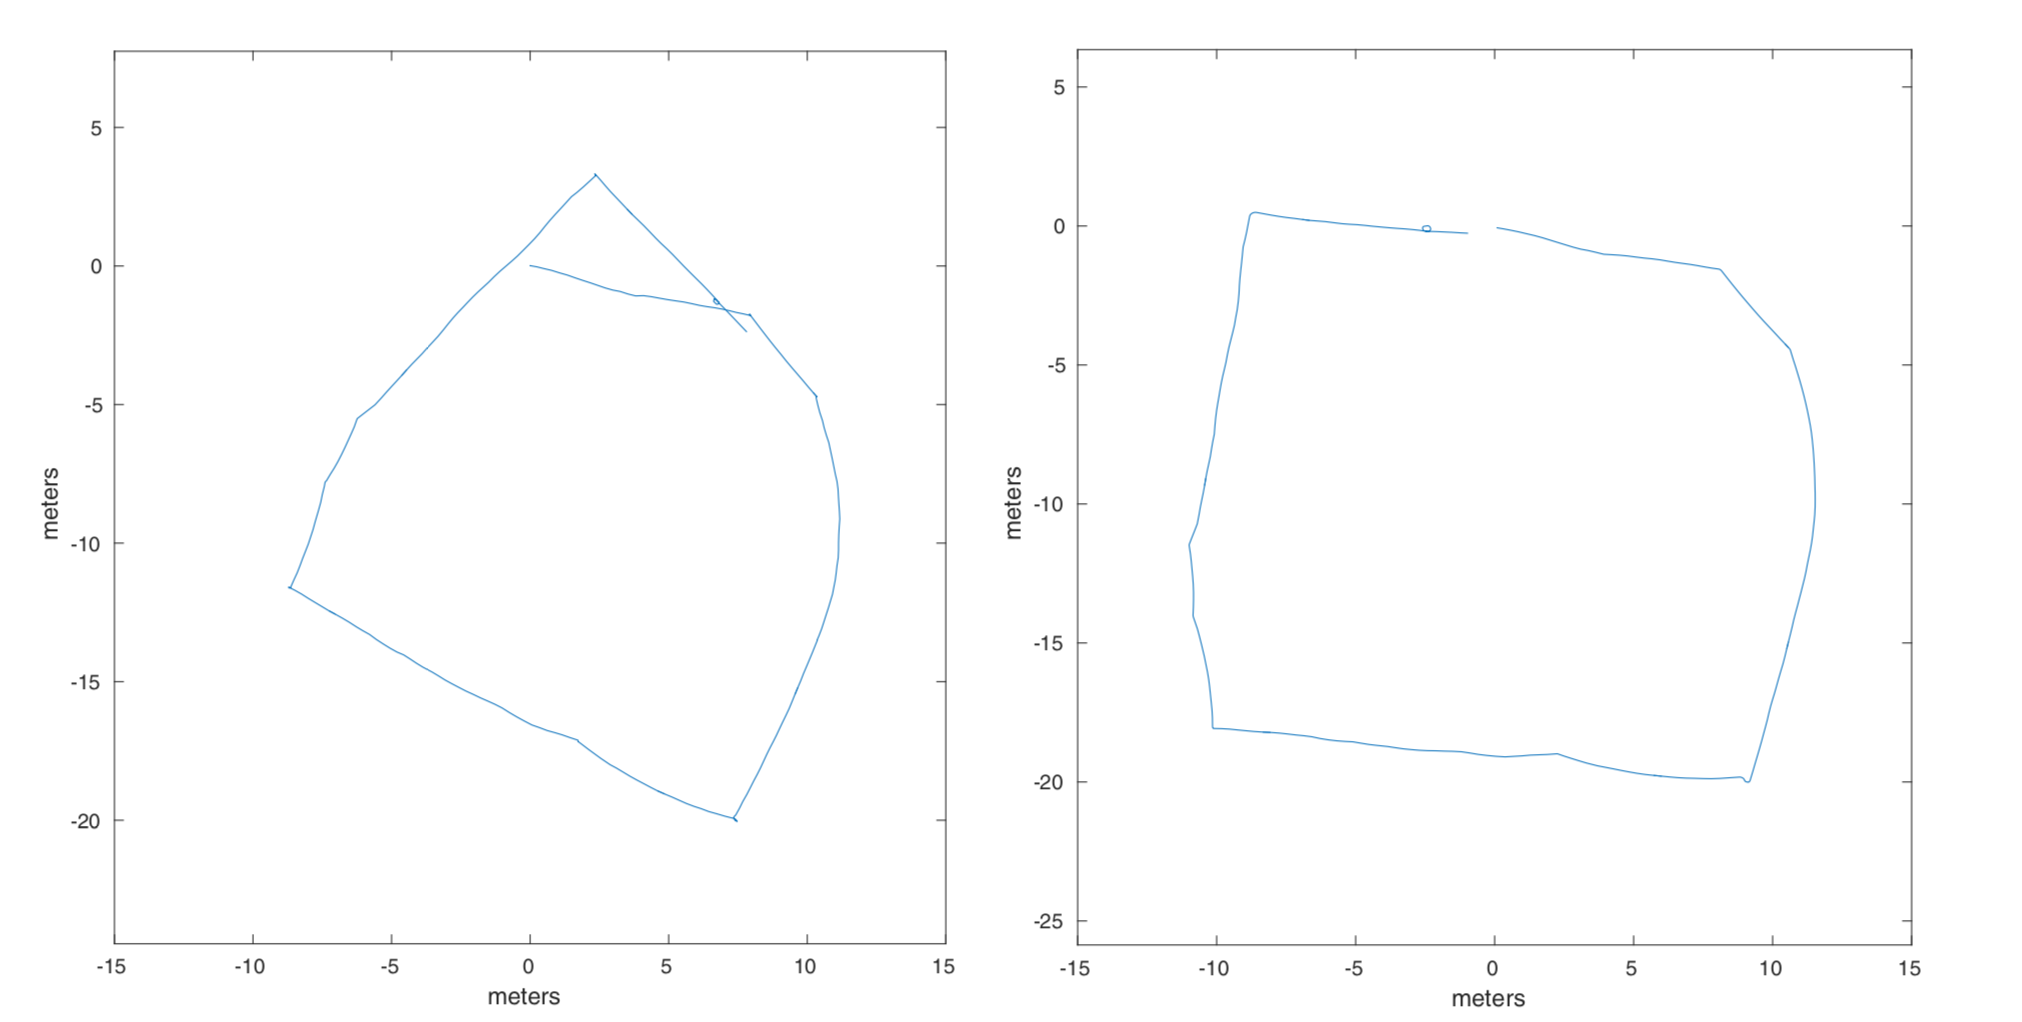
\includegraphics[width=8cm]{./images/example_input_and_output.png}
    \caption{Example input (left) and output state vector (right) of the GraphSLAM algorithm}\label{fig:sim-in-and-out}
\end{figure}
この画像には地図が描かれていないが、ロボットが移動した軌跡を示す。右側は正方形の図形を示しており、実際の建物の構造に一致している。
データセットのオドメトリデータはICPアルゴリズムで修正されており、GraphSLAMでループを閉じた結果、オドメトリのみでの場合と比較して状態推定が良好になった。
一方、修正前のオドメトリは、ループを閉じた後も状態推定において誤差が収束することはなかった。
ICPアルゴリズムで修正したオドメトリの状態ベクトルのループを閉じることは、修正されていない状態ベクトルよりも容易である。

\subsection{実機への実装}
\ref{sec:approach}章にて示した手法を用いて実際にAltera社のFPGAであるCyclone V上にC$\lambda$aSHを用いてGraphSLAMを決定論的に構築した。
このアーキテクチャに対応する合成結果を表\ref{tab:fpga-results}に示す。
% Cyclone Vは110000の論理素子、112のDSP、5140kbitのblockRAMを持つ。
\begin{table}[H]
\caption{FPGA SYNTHESIS RESULTS}
\begin{tabular}{|l|r|r|r|}
\hline
               & Used    & Available & Utilization \\ \hline
ALMs           & 2611    & 41,910    & 6\%         \\
BlockRAM(bits) & 412,784 & 5,662,720 & 7\%         \\
DSPs           & 8       & 112       & 7\%         \\ \hline
\end{tabular}
\label{tab:fpga-results}
\end{table}
システムは15bitの整数ビットと12bitの小数ビットで構成される27bit符号付き固定小数点データ型を使用してシミュレートされ、合成された。
ベクトルALUは、8つの計算を並列に実行する算術演算ユニットとしてシミュレートされ、合成された。
表\ref{tab:fpga-results}の合成結果が示す27bitDSPの数に等しい。


\section{結言}
FPGA上にGraphSLAMアルゴリズムを実装するために使用する方法論を示した。
C$\lambda$aSHを用いて数学的記述を低級なハードウェア記述に変換し、FPGA上にGraphSLAMを実装した。
設計時間を定量化することは難しい問題であるが、
従来の方法ではハードウェアアーキテクチャの開発に膨大な時間がかかるSLAMのような大規模なアプリケーションに対して
C$\lambda$aSHによる抽象化で開発を大幅に簡略化することができた。

\subsection{今後の展望}
面積-時間トレードオフを手作業で行ったが、これは時間のかかるプロセスである。
リソースと並列化性能の観点からハードウェアの性能限界とアルゴリズムをパラメータ化することにより、
設計がパラメータ化可能であれば、面積-時間トレードオフを自動的に行うことができ、さらなる設計時間の短縮が可能である。

\footnotesize
\bibliographystyle{citarlab}
\bibliography{./references}

\normalsize
\end{document}
